\documentclass[12pt,a4paper]{article}

% ==============================================================================
% GÓI THƯ VIỆN CƠ BẢN VÀ HỖ TRỢ TIẾNG VIỆT
% ==============================================================================
\usepackage[utf8]{inputenc}
\usepackage[T5]{fontenc}
\usepackage[vietnamese]{babel}

\usepackage{amsmath, amssymb, amsthm, mathtools}
\usepackage{graphicx}
\usepackage{xcolor}
\usepackage{booktabs, multirow, makecell, tabularx, longtable, array}
\usepackage{geometry}
\geometry{
    a4paper,
    left=25mm,
    right=20mm,
    top=25mm,
    bottom=25mm
}
\usepackage{fancyhdr}
\usepackage{titlesec}
\usepackage{enumitem}
\usepackage{listings}
\usepackage{tcolorbox}
\tcbuselibrary{breakable}
\usepackage{hyperref}
\usepackage{tikz}
\usepackage{float}

% Cấu hình đường dẫn thư mục ảnh
\graphicspath{{./}{figures/}}

% Cấu hình Hyperlink
\hypersetup{
    colorlinks=true,
    linkcolor=blue!75!black,
    citecolor=red!75!black,
    urlcolor=teal!80!black
}

% Cấu hình Header & Footer
\setlength{\headheight}{15pt}
\addtolength{\topmargin}{-3pt}
\pagestyle{fancy}
\fancyhf{}
\fancyhead[L]{\small\textit{Học viện Công nghệ Bưu chính Viễn thông -- PTIT}}
\fancyhead[R]{\small\textit{Báo cáo Kỹ thuật Assignment 06 -- LTHTTM}}
\fancyfoot[C]{\thepage}
\renewcommand{\headrulewidth}{0.6pt}
\renewcommand{\footrulewidth}{0.4pt}

% Cấu hình Code Listing
\lstset{
    language=Python,
    basicstyle=\ttfamily\footnotesize,
    keywordstyle=\color{blue!80!black}\bfseries,
    commentstyle=\color{green!50!black}\itshape,
    stringstyle=\color{red!70!black},
    numbers=left,
    numberstyle=\tiny\color{gray},
    stepnumber=1,
    numbersep=8pt,
    backgroundcolor=\color{gray!5},
    frame=single,
    rulecolor=\color{gray!30},
    breaklines=true,
    breakatwhitespace=true,
    showstringspaces=false,
    tabsize=4
}

% Định dạng tiêu đề các mục
\titleformat{\section}{\large\bfseries\color{blue!85!black}}{\thesection}{1em}{}[\titlerule]
\titleformat{\subsection}{\normalsize\bfseries\color{cyan!75!black}}{\thesubsection}{1em}{}
\titleformat{\subsubsection}{\small\bfseries\color{black}}{\thesubsubsection}{1em}{}

% Khối ghi chú nổi bật
\newtcolorbox{mybox}[1]{
    colback=blue!5!white,
    colframe=blue!75!black,
    fonttitle=\bfseries,
    title=#1,
    arc=2mm,
    boxrule=1pt
}

% Khối chú thích & phân tích biểu đồ chuyên sâu
\newtcolorbox{chartbox}[1][]{
    colback=blue!2!white,
    colframe=blue!70!black,
    fonttitle=\bfseries\small,
    coltitle=white,
    arc=1.5mm,
    boxrule=0.8pt,
    left=3mm,
    right=3mm,
    top=2mm,
    bottom=2mm,
    breakable,
    title=#1
}

% Cấu hình cột bảng tự co giãn và căn lề
\newcolumntype{L}[1]{>{\raggedright\arraybackslash}p{#1}}
\newcolumntype{C}[1]{>{\centering\arraybackslash}p{#1}}
\newcolumntype{Y}{>{\centering\arraybackslash}X}

% ==============================================================================
% BẮT ĐẦU TÀI LIỆU
% ==============================================================================
\begin{document}

% ==============================================================================
% TRANG BÌA CHUẨN KHUNG VIỀN CỔ ĐIỂN VÀ HỌA TIẾT 4 GÓC THEO FILE DOCX
% ==============================================================================
\begin{titlepage}
    \begin{tikzpicture}[remember picture, overlay]
        % 1. Đường viền khung ngoài dày
        \draw[line width=2.2pt, color=black]
            ([xshift=15mm, yshift=-15mm]current page.north west)
            rectangle
            ([xshift=-15mm, yshift=15mm]current page.south east);
        
        % 2. Đường viền khung trong mảnh
        \draw[line width=0.8pt, color=black]
            ([xshift=17.5mm, yshift=-17.5mm]current page.north west)
            rectangle
            ([xshift=-17.5mm, yshift=17.5mm]current page.south east);
    \end{tikzpicture}

    \centering
    \vspace*{0.2cm}
    {\large \textbf{HỌC VIỆN CÔNG NGHỆ BƯU CHÍNH VIỄN THÔNG}}\\[0.25cm]
    {\large \textbf{KHOA CÔNG NGHỆ THÔNG TIN 1}}\\[0.2cm]
    \rule{5cm}{1pt}\\[0.9cm]

    % Logo PTIT
    \begin{center}
        \IfFileExists{figures/logo_ptit.png}{%
            
\includegraphics[width=3.4cm, height=4.2cm, keepaspectratio]{figures/logo_ptit.png}
        }{%
            \begin{tcolorbox}[colback=red!5!white, colframe=red!75!black, width=3.8cm, height=3.8cm, arc=2mm, halign=center, valign=center]
                \Large \textbf{\color{red!80!black}PTIT}\\[0.1cm]
                \footnotesize \textbf{\color{black}LOGO}
            \end{tcolorbox}
        }
    \end{center}

    \vspace{0.6cm}

    {\Large \textbf{BÁO CÁO KỸ THUẬT ASSIGNMENT 06}}\\[0.3cm]
    {\large \textbf{MÔN HỌC: LẬP TRÌNH HỆ THỐNG THÔNG MINH}}\\[0.5cm]
    {\Large \textbf{\color{blue!85!black}MẠNG NƠ-RON HỒI QUY (RNN) TỪ CƠ SỞ LÝ THUYẾT ĐẾN ỨNG DỤNG DỰ BÁO CHUỖI THỜI GIAN}}\\[0.3cm]
    {\normalsize \textit{Nghiên cứu Giải tích, Hiện thực Hóa Mã nguồn thuần (NumPy) và Đối chuẩn Thực nghiệm trên Keras và PyTorch (Gold Price, AMZN)}}

    \vspace{0.8cm}

    \begin{flushleft}
        \hspace{1.6cm}
        \begin{tabular}{p{5.0cm} p{0.5cm} l}
            \textbf{Giảng viên hướng dẫn} & : & \textbf{PGS.TS. Trần Đình Quế} \\[0.3cm]
            \textbf{Lớp}                  & : & \textbf{D23CTPM01} \\[0.3cm]
            \textbf{Nhóm học phần}        & : & \textbf{CT01} \\[0.3cm]
            \textbf{Thành viên thực hiện} & : & \textbf{Nguyễn Nam Hải} \\[0.3cm]
            \textbf{Mã sinh viên}         & : & \textbf{B23DCCN277} \\[0.3cm]
        \end{tabular}
    \end{flushleft}

    \vfill
    {\large \textbf{Hà Nội -- 2026}}
    \vspace*{0.3cm}
\end{titlepage}

% ==============================================================================
% MỤC LỤC BÁO CÁO KỸ THUẬT
% ==============================================================================
\newpage
\renewcommand{\contentsname}{MỤC LỤC BÁO CÁO KỸ THUẬT ASSIGNMENT 06}
\tableofcontents
\newpage

% ==============================================================================
% DANH MỤC HÌNH VẼ & BẢNG BIỂU
% ==============================================================================
\phantomsection
\addcontentsline{toc}{section}{DANH MỤC HÌNH VẼ}
\listoffigures

\vspace{0.8cm}

\phantomsection
\addcontentsline{toc}{section}{DANH MỤC BẢNG BIỂU}
\listoftables

\newpage

% ==============================================================================
% TÓM TẮT BÁO CÁO (ABSTRACT)
% ==============================================================================
\phantomsection
\addcontentsline{toc}{section}{TÓM TẮT BÁO CÁO (ABSTRACT)}
\section*{TÓM TẮT BÁO CÁO (ABSTRACT)}

Báo cáo Kỹ thuật Assignment 06 trình bày nghiên cứu hệ thống và khảo sát thực nghiệm chuyên sâu về Mạng nơ-ron Hồi quy (Recurrent Neural Network -- RNN). Mục tiêu của báo cáo là hệ thống hóa toàn bộ vòng đời phát triển của một bài toán Deep Learning dành riêng cho chuỗi thời gian: từ khâu am hiểu cơ sở toán học thuần túy, phân tích khám phá đặc trưng phân phối dữ liệu (EDA), cho đến hiện thực hóa mã nguồn (bằng NumPy, PyTorch, Keras) và cuối cùng là triển khai lên một hệ thống Web Dashboard hoàn chỉnh.

Báo cáo phân tích sâu sắc các rào cản kinh điển của chuỗi thời gian như: Tại sao mạng MLP hay Conv1D không đủ năng lực xử lý? Ma trận Jacobian ảnh hưởng như thế nào đến sự suy thoái Gradient? Làm thế nào để giải quyết bằng kỹ thuật Gradient Clipping? Thông qua việc đối chuẩn trên 2 tập dữ liệu tài chính thực tế (Gold Price và AMZN Stock), báo cáo đã bóc tách rõ ràng hiện tượng "Trễ pha" (Lagging) - một đặc trưng của Vanilla RNN khi cố gắng mô phỏng một quy luật bước đi ngẫu nhiên (Random Walk) trên thị trường tài chính.

\newpage

% ==============================================================================
% CHƯƠNG 1
% ==============================================================================
\section{Cơ sở lý thuyết giải tích và toán học của mạng nơ-ron hồi quy (RNN)}

\subsection{Dữ liệu tuần tự và không gian biểu diễn Tensor ba chiều}
Trong học sâu (Deep Learning), dữ liệu tuần tự (Sequential Data) nói chung và chuỗi thời gian (Time-series Data) nói riêng sở hữu đặc thù cấu trúc mang tính định hướng: \textbf{Thứ tự xuất hiện của các phần tử mang thông tin nhân quả và ngữ cảnh quyết định}. Xét một chuỗi quan sát \(X = \{x_1, x_2, \dots, x_T\}\), tại mỗi thời điểm \(t\), giá trị của \(x_t\) không tồn tại độc lập mà bị chi phối bởi toàn bộ lịch sử các quan sát phía trước nó \(\{x_\tau\}_{\tau=1}^{t-1}\). 

Để các thư viện tính toán ma trận (như NumPy, PyTorch, TensorFlow) có thể tối ưu hóa thông qua các phép nhân khối (Block Matrix Multiplication) trên phần cứng tăng tốc (GPU/TPU), dữ liệu chuỗi được cấu trúc hóa thành một \textbf{Tensor 3 chiều} có dạng chuẩn \((B, T, D)\):
\begin{itemize}[leftmargin=*]
    \item \textbf{Batch Size (\(B\)):} Số lượng chuỗi con (sequences) độc lập được đưa vào tính toán đồng thời trong một lượt lan truyền nhằm giảm thiểu phương sai của gradient ước lượng.
    \item \textbf{Sequence Length (\(T\)):} Chiều dài thời gian của cửa sổ trượt (Time Window). Đây là số lượng time-steps mà mạng hồi quy phải duyệt qua liên tiếp.
    \item \textbf{Input Dimension / Feature Size (\(D\)):} Số lượng biến/đặc trưng đo lường tại mỗi mốc thời gian \(t\). Trong bài toán chuỗi thời gian đơn biến (Univariate Time-series, ví dụ như giá đóng cửa của Vàng hoặc AMZN), \(D = 1\). Đối với bài toán đa biến (Multivariate), \(D\) có thể mở rộng bao gồm giá mở cửa, khối lượng giao dịch, các chỉ báo kỹ thuật RSI, MACD, v.v.
\end{itemize}

\subsection{Phân loại các cấu trúc bài toán chuỗi thời gian}
Dựa trên sự tương quan chiều giữa chuỗi đầu vào và chuỗi đầu ra, các kiến trúc hồi quy được chuẩn hóa thành bốn mô hình tính toán hình thái:
\begin{enumerate}[leftmargin=*]
    \item \textbf{One-to-One:} Không gian đầu vào và đầu ra đều là vector tĩnh (\(T_{in} = 1, T_{out} = 1\)). Đây thực chất là mô hình mạng truyền thẳng (Feedforward Neural Network - MLP) cổ điển, không lưu vết trạng thái lịch sử.
    \item \textbf{One-to-Many:} Mạng nhận một vector đặc trưng duy nhất tại \(t=1\) và sinh ra một chuỗi đầu ra có độ dài biến thiên \(T_{out} > 1\) (tiêu biểu như bài toán chú thích hình ảnh - Image Captioning, sinh nhạc tự động).
    \item \textbf{Many-to-One:} Mạng nhận một chuỗi đầu vào \(\{x_1, x_2, \dots, x_T\}\) và chỉ sinh ra một giá trị dự báo duy nhất \(\hat{y}\) tại mốc thời gian cuối cùng \(T\). \textbf{Đây là cấu trúc nền tảng được triển khai trong nghiên cứu này}, nơi mô hình đọc chuỗi giá 30 ngày trong quá khứ để dự báo giá trị của ngày thứ 31.
    \item \textbf{Many-to-Many:} Bao gồm hai biến thể kiến trúc:
    \begin{itemize}
        \item \textit{Đồng bộ (Synchronized):} Chiều dài chuỗi vào và ra bằng nhau (\(T_{in} = T_{out}\)), mỗi bước \(t\) tiếp nhận \(x_t\) sẽ lập tức sinh ra một đầu ra \(y_t\) tương ứng (như bài toán gán nhãn từ loại POS tagging, phát hiện bất thường thời gian thực).
        \item \textit{Bất đồng bộ (Encoder - Decoder / Seq2Seq):} Chiều dài vào và ra không nhất thiết bằng nhau (\(T_{in} \neq T_{out}\)). Toàn bộ thông tin chuỗi nguồn được mạng Encoder nén vào một vector ngữ cảnh (Context Vector), trước khi mạng Decoder giải nén để sinh chuỗi đích (như trong dịch máy, nhận dạng giọng nói).
    \end{itemize}
\end{enumerate}

\subsection{Sự bất cập của MLP và mạng nơ-ron tích chập 1 chiều (Conv1D)}
Trước khi mạng hồi quy được ứng dụng rộng rãi, hai phương pháp truyền thống thường được áp dụng để giải quyết chuỗi thời gian là mạng truyền thẳng đa tầng (MLP) và mạng tích chập 1 chiều (Conv1D). Tuy nhiên, cả hai đều bộc lộ những rào cản lý thuyết nghiêm ngặt:
\begin{itemize}[leftmargin=*]
    \item \textbf{Mạng truyền thẳng đa tầng (MLP):} Bắt buộc phải dàn phẳng (flatten) chuỗi \((T, D)\) thành một vector duy nhất có kích thước \(T \times D\). Cách tiếp cận này vi phạm tính bất biến tịnh tiến theo thời gian (Temporal Translation Invariance). Trọng số kết nối với ngày thứ $1$ hoàn toàn độc lập với trọng số kết nối với ngày thứ $30$. Do đó, nếu một mô hình giá (chart pattern) xuất hiện ở đầu chuỗi, MLP không thể tái sử dụng tri thức đó khi mô hình tương tự lặp lại ở cuối chuỗi. Hơn nữa, số lượng tham số bùng nổ theo chiều dài \(T\) khiến mô hình rất dễ rơi vào tình trạng quá khớp (Overfitting).
    \item \textbf{Mạng tích chập 1 chiều (Conv1D):} Sử dụng các bộ lọc trượt trên trục thời gian, đảm bảo được tính chia sẻ tham số (Parameter Sharing). Tuy nhiên, trường tiếp nhận (Receptive Field) của Conv1D bị giới hạn nghiêm ngặt bởi kích thước hạt nhân (Kernel Size) và số lớp tích chập. Để ghi nhận phụ thuộc xa, mạng buộc phải xếp chồng nhiều tầng hoặc dùng tích chập giãn nở (Dilated Convolution). Dẫu vậy, Conv1D không duy trì một bộ nhớ nội tại mang tính liên tục để lưu vết trạng thái tích lũy của toàn bộ chuỗi.
\end{itemize}

\subsection{Kiến trúc Vanilla RNN và cơ chế chia sẻ tham số (Parameter Sharing)}
Mạng nơ-ron hồi quy đơn giản (Vanilla RNN) giải quyết triệt để các hạn chế trên bằng cách đưa vào khái niệm \textbf{Trạng thái ẩn (Hidden State - \(h_t\))}. Trạng thái ẩn tại bước \(t\) đóng vai trò như một bộ nhớ động, tổng hợp thông tin từ đầu vào hiện tại \(x_t\) và trạng thái ẩn tích lũy của bước liền trước \(h_{t-1}\).

Điểm mấu chốt mang lại sức mạnh khái quát hóa cho RNN là \textbf{nguyên lý chia sẻ tham số}: Cùng một bộ ma trận trọng số \((W, U, V)\) và vector độ lệch \((b_h, b_y)\) được tái sử dụng tại tất cả các bước thời gian \(t = 1, 2, \dots, T\).

\begin{figure}[htbp]
    \centering
    \begin{tikzpicture}[scale=0.85, every node/.style={transform shape}]
        % Sơ đồ dạng cuộn (Folded)
        \node[draw, rectangle, rounded corners, minimum width=1.5cm, minimum height=1cm, fill=blue!10] (cell) at (0,2) {\(h_t\)};
        \node (x) at (0,0) {\(x_t\)};
        \node (y) at (0,4) {\(\hat{y}_t\)};
        \draw[->, thick] (x) -- node[right] {\(W\)} (cell);
        \draw[->, thick] (cell) -- node[right] {\(V\)} (y);
        \draw[->, thick] (cell) to [out=150,in=210,looseness=4] node[left] {\(U\)} (cell);
        \node at (0, -1) {\textbf{(a) Dạng cuộn (Folded)}};

        % Dấu mũi tên unroll
        \draw[->, very thick, dashed] (1.8, 2) -- (3.2, 2);
        \node at (2.5, 2.4) {\footnotesize Unroll};

        % Sơ đồ dạng trải phẳng (Unrolled)
        \node[draw, rectangle, rounded corners, minimum width=1.2cm, minimum height=0.9cm, fill=blue!10] (h1) at (4.5,2) {\(h_{t-1}\)};
        \node[draw, rectangle, rounded corners, minimum width=1.2cm, minimum height=0.9cm, fill=blue!10] (h2) at (7.5,2) {\(h_t\)};
        \node[draw, rectangle, rounded corners, minimum width=1.2cm, minimum height=0.9cm, fill=blue!10] (h3) at (10.5,2) {\(h_{t+1}\)};

        \node (x1) at (4.5,0) {\(x_{t-1}\)};
        \node (x2) at (7.5,0) {\(x_t\)};
        \node (x3) at (10.5,0) {\(x_{t+1}\)};

        \node (y1) at (4.5,4) {\(\hat{y}_{t-1}\)};
        \node (y2) at (7.5,4) {\(\hat{y}_t\)};
        \node (y3) at (10.5,4) {\(\hat{y}_{t+1}\)};

        \draw[->, thick] (x1) -- node[right] {\(W\)} (h1);
        \draw[->, thick] (x2) -- node[right] {\(W\)} (h2);
        \draw[->, thick] (x3) -- node[right] {\(W\)} (h3);

        \draw[->, thick] (h1) -- node[above] {\(U\)} (h2);
        \draw[->, thick] (h2) -- node[above] {\(U\)} (h3);
        \draw[->, thick] (3.2, 2) -- (h1);
        \draw[->, thick] (h3) -- (11.8, 2);

        \draw[->, thick] (h1) -- node[right] {\(V\)} (y1);
        \draw[->, thick] (h2) -- node[right] {\(V\)} (y2);
        \draw[->, thick] (h3) -- node[right] {\(V\)} (y3);
        \node at (7.5, -1) {\textbf{(b) Dạng trải phẳng theo thời gian (Unrolled)}};
    \end{tikzpicture}
    \caption{Cấu trúc toán học của mạng Vanilla RNN: dạng cuộn gọn và dạng trải phẳng theo thời gian.}
    \label{fig:rnn_unroll}
\end{figure}

Quá trình lan truyền xuôi (Forward Pass) được chuẩn hóa qua hệ phương trình đại số tuyến tính:
\begin{align}
    a_t &= W x_t + U h_{t-1} + b_h \label{eq:pre_activation} \\
    h_t &= \tanh(a_t) \label{eq:hidden_state} \\
    \hat{y}_t &= V h_t + b_y \label{eq:output}
\end{align}
Trong đó:
\begin{itemize}[leftmargin=*]
    \item \(x_t \in \mathbb{R}^{D \times 1}\) là vector đặc trưng đầu vào tại bước \(t\).
    \item \(h_t \in \mathbb{R}^{H \times 1}\) là trạng thái ẩn tại bước \(t\) (\(H\) là số chiều ẩn - Hidden Dimension).
    \item \(W \in \mathbb{R}^{H \times D}\) là ma trận trọng số biến đổi từ đầu vào sang trạng thái ẩn.
    \item \(U \in \mathbb{R}^{H \times H}\) là ma trận trọng số hồi quy chuyển đổi từ \(h_{t-1}\) sang \(h_t\).
    \item \(V \in \mathbb{R}^{K \times H}\) là ma trận trọng số biến đổi từ trạng thái ẩn sang đầu ra dự báo (\(K\) là chiều đầu ra, với bài toán đơn biến dự báo 1 bước, \(K=1\)).
    \item \(b_h \in \mathbb{R}^{H \times 1}\) và \(b_y \in \mathbb{R}^{K \times 1}\) là các vector độ lệch tương ứng.
    \item Hàm kích hoạt \(\tanh(z) = \frac{e^z - e^{-z}}{e^z + e^{-z}}\) có miền giá trị chặt trong khoảng \((-1, 1)\), giúp kiểm soát biên độ phân kỳ của trạng thái ẩn qua các chu kỳ hồi quy.
\end{itemize}

\subsection{Khai triển giải tích BPTT (Backpropagation Through Time)}
Trong cấu trúc dự báo Many-to-One, hàm mất mát chỉ được tính tại thời điểm cuối cùng \(T\). Xét hàm mất mát sai số bình phương trung bình (MSE) cho một mẫu huấn luyện:
\begin{equation}
    \mathcal{L} = \frac{1}{2} \|\hat{y}_T - y_{true}\|_2^2 = \frac{1}{2} (\hat{y}_T - y_{true})^T (\hat{y}_T - y_{true})
\end{equation}

\subsubsection{Gradient tại tầng đầu ra (Output Layer)}
Áp dụng quy tắc chuỗi cho tầng ra tại bước \(T\):
\begin{align}
    d\hat{y}_T &= \frac{\partial \mathcal{L}}{\partial \hat{y}_T} = \hat{y}_T - y_{true} \in \mathbb{R}^{K \times 1} \\
    \frac{\partial \mathcal{L}}{\partial V} &= d\hat{y}_T \cdot h_T^T \in \mathbb{R}^{K \times H} \\
    \frac{\partial \mathcal{L}}{\partial b_y} &= d\hat{y}_T \in \mathbb{R}^{K \times 1}
\end{align}
Sai số truyền ngược từ tầng ra vào trạng thái ẩn cuối cùng \(h_T\):
\begin{equation}
    \delta_T = \frac{\partial \mathcal{L}}{\partial h_T} = V^T \cdot d\hat{y}_T \in \mathbb{R}^{H \times 1}
\end{equation}

\subsubsection{Lan truyền ngược qua dòng thời gian}
Bởi vì ma trận \(W\), \(U\) và \(b_h\) xuất hiện ở mọi bước thời gian từ \(t=1\) đến \(t=T\), đạo hàm toàn phần của hàm mất mát theo các tham số này là tổng tích lũy của các đạo hàm thành phần tại từng bước thời gian:
\begin{equation}
    \frac{\partial \mathcal{L}}{\partial W} = \sum_{t=1}^{T} \left. \frac{\partial \mathcal{L}}{\partial W} \right|_t, \quad 
    \frac{\partial \mathcal{L}}{\partial U} = \sum_{t=1}^{T} \left. \frac{\partial \mathcal{L}}{\partial U} \right|_t, \quad 
    \frac{\partial \mathcal{L}}{\partial b_h} = \sum_{t=1}^{T} \left. \frac{\partial \mathcal{L}}{\partial b_h} \right|_t
\end{equation}

Tại một bước thời gian \(t\) bất kỳ (\(1 \le t \le T\)), gọi \(\delta_t = \frac{\partial \mathcal{L}}{\partial h_t}\). Gradient lan truyền qua hàm phi tuyến \(\tanh\) tại nút tiền kích hoạt \(a_t\):
\begin{equation}
    \delta_t^{raw} = \frac{\partial \mathcal{L}}{\partial a_t} = \delta_t \odot \tanh'(a_t) = \delta_t \odot (1 - h_t^2)
\end{equation}
trong đó \(\odot\) biểu thị tích Hadamard (element-wise product) và sử dụng đồng nhất thức \(\tanh'(z) = 1 - \tanh^2(z)\).

Khi đó, gradient tích lũy tại bước \(t\) được xác định:
\begin{align}
    dW_t &= \delta_t^{raw} \cdot x_t^T \in \mathbb{R}^{H \times D} \\
    dU_t &= \delta_t^{raw} \cdot h_{t-1}^T \in \mathbb{R}^{H \times H} \quad (\text{với } h_0 = \mathbf{0}) \\
    db_{h, t} &= \delta_t^{raw} \in \mathbb{R}^{H \times 1}
\end{align}

Để tiếp tục lan truyền ngược về bước \(t-1\), ta tính đạo hàm theo \(h_{t-1}\):
\begin{equation}
    \delta_{t-1} = \frac{\partial \mathcal{L}}{\partial h_{t-1}} = \left( \frac{\partial a_t}{\partial h_{t-1}} \right)^T \frac{\partial \mathcal{L}}{\partial a_t} = U^T \cdot \delta_t^{raw} = U^T \left( \delta_t \odot (1 - h_t^2) \right)
\end{equation}

\subsection{Bản chất suy thoái (Vanishing) và bùng nổ (Exploding) Gradient: Khảo sát ma trận Jacobian}
Vấn đề cốt tử của BPTT được bộc lộ rõ ràng khi ta phân tích gradient lan truyền từ bước cuối \(T\) về một bước \(k\) nằm xa trong quá khứ (\(k \ll T\)):
\begin{equation}
    \delta_k = \frac{\partial \mathcal{L}}{\partial h_k} = \frac{\partial \mathcal{L}}{\partial h_T} \frac{\partial h_T}{\partial h_k} = \delta_T \prod_{j=k+1}^{T} \frac{\partial h_j}{\partial h_{j-1}}
\end{equation}
Ma trận Jacobian trung gian giữa hai trạng thái ẩn liên tiếp có dạng:
\begin{equation}
    J_j = \frac{\partial h_j}{\partial h_{j-1}} = \text{diag}(1 - h_j^2) U^T
\end{equation}
Khai triển tích chuỗi ma trận:
\begin{equation}
    \frac{\partial h_T}{\partial h_k} = \prod_{j=k+1}^{T} \text{diag}(1 - h_j^2) U^T
\end{equation}

Đánh giá chuẩn ma trận (Matrix Norm) theo tính chất bất đẳng thức Schwarz:
\begin{equation}
    \left\| \frac{\partial h_T}{\partial h_k} \right\| \le \prod_{j=k+1}^{T} \|\text{diag}(1 - h_j^2)\| \cdot \|U^T\|
\end{equation}
Ta xét hai thành phần nhân tử:
\begin{enumerate}[leftmargin=*]
    \item \textbf{Thành phần phi tuyến:} Do đạo hàm của hàm hyperbolic tangent bị chặn trên: \(0 < 1 - h_j^2 \le 1\), nên \(\|\text{diag}(1 - h_j^2)\| \le 1\). Dấu bằng chỉ xảy ra khi \(h_j = 0\). Càng xa điểm cân bằng, nhân tử này càng nhỏ hơn 1.
    \item \textbf{Thành phần ma trận hồi quy:} Gọi \(\rho(U)\) là bán kính phổ (Spectral Radius - giá trị riêng lớn nhất theo trị tuyệt đối) của \(U\). Theo định lý Gelfand, \(\|U^m\| \approx \rho(U)^m\) khi \(m = T - k\) lớn.
\end{enumerate}

Từ đây phát sinh hai thái cực bất ổn định số học:
\begin{mybox}{Nghịch lý toán học trong BPTT của Vanilla RNN}
\begin{itemize}[leftmargin=*]
    \item \textbf{Bùng nổ Gradient (Exploding Gradient):} Xảy ra khi $\rho(U) > 1$ và các trạng thái \(h_j\) không rơi vào vùng bão hòa của \(\tanh\). Tích ma trận \(U^{T-k}\) tăng trưởng theo quy luật hàm mũ, khiến \(\|\delta_k\| \to \infty\). Hệ quả là các trọng số bị cập nhật với bước nhảy khổng lồ, làm tràn số (NaN/Inf) và phá vỡ hoàn toàn quỹ đạo hội tụ.
    \item \textbf{Triệt tiêu / Suy thoái Gradient (Vanishing Gradient):} Xảy ra khi \(\rho(U) < 1\) hoặc khi trạng thái ẩn \(h_j\) tiến sát \(\pm 1\) khiến \(\tanh'(a_j) = 1 - h_j^2 \to 0\) (hiện tượng bão hòa hàm kích hoạt). Khi đó, \(\lim_{T-k \to \infty} \left\| \frac{\partial h_T}{\partial h_k} \right\| = 0\). Gradient tại các mốc thời gian ban đầu tiệm cận về 0, đồng nghĩa với việc mạng không thể học được bất kỳ mối liên hệ dài hạn nào vượt quá 10--15 bước thời gian.
\end{itemize}
\end{mybox}

\subsection{Các giải pháp kỹ thuật ổn định hóa Gradient trong Vanilla RNN}

\subsubsection{Cắt tỉa Gradient (Gradient Clipping)}
Kỹ thuật Gradient Clipping theo chuẩn L2 (Global Norm Clipping) được đề xuất bởi Pascanu et al. (2013) nhằm giải quyết dứt điểm hiện tượng bùng nổ đạo hàm. Thay vì cắt xén độc lập từng phần tử (làm méo mó hướng của gradient vector), thuật toán giám sát chuẩn tổng thể của toàn bộ tham số:
\begin{equation}
    g = \left[ \text{vec}(dW), \text{vec}(dU), \text{vec}(dV), \text{vec}(db_h), \text{vec}(db_y) \right]^T
\end{equation}
Nếu \(\|g\|_2 > \gamma\) (với \(\gamma\) là ngưỡng cắt tỉa - clipping threshold, thường chọn \(\gamma = 1.0\) hoặc $5.0$), vector gradient được co rút theo tỷ lệ:
\begin{equation}
    g \leftarrow g \cdot \frac{\gamma}{\|g\|_2}
\end{equation}
Phép biến đổi này bảo toàn hoàn toàn vector chỉ phương của gradient trong không gian tham số, đồng thời giới hạn bước nhảy tối đa của thuật toán tối ưu, loại trừ hoàn toàn nguy cơ phân kỳ do nổ gradient.

\subsubsection{Khởi tạo trọng số trực giao (Orthogonal Initialization)}
Để giảm thiểu triệt tiêu gradient mà không cần thay đổi cấu trúc mạng, ma trận hồi quy \(U\) được khởi tạo thỏa mãn tính chất trực giao:
\begin{equation}
    U^T U = I \implies \|U x\|_2 = \|x\|_2, \quad \forall x \in \mathbb{R}^H
\end{equation}
Tất cả các giá trị riêng của ma trận trực giao đều có độ lớn chính xác bằng 1 (\(|\lambda_i| = 1\)). Nhờ đó, khi gradient truyền ngược qua phép nhân \(U^T\), biên độ của vector sai số không bị co rút hay phình to một cách nhân tạo do ảnh hưởng của ma trận trọng số, giúp thông tin gradient có thể truyền sâu hơn qua chuỗi thời gian dài.

\subsubsection{Giới hạn cố hữu và bước đệm chuyển dịch sang LSTM/GRU}
Mặc dù Gradient Clipping và Orthogonal Initialization giúp ổn định quá trình huấn luyện, chúng không thể giải quyết triệt để vấn đề suy thoái gradient gây ra bởi đạo hàm \(1 - h_t^2\) của hàm \(\tanh\). 

Đây là giới hạn cấu trúc cố hữu của Vanilla RNN, đặt ra yêu cầu tất yếu cho sự ra đời của các kiến trúc cổng nhớ (Gated RNN) như \textbf{LSTM (Long Short-Term Memory)} và \textbf{GRU (Gated Recurrent Unit)}. Bằng việc đưa vào đường truyền trạng thái ô nhớ tuyến tính (Constant Error Carousel - CEC):
\begin{equation}
    C_t = f_t \odot C_{t-1} + i_t \odot \tilde{C}_t
\end{equation}
đạo hàm \(\frac{\partial C_t}{\partial C_{t-1}} = f_t\) không còn bị chi phối bởi tích ma trận liên tiếp, cho phép gradient lan truyền nguyên vẹn qua hàng trăm bước thời gian.


% ==============================================================================
% CHƯƠNG 2
% ==============================================================================
\section{Khảo sát dữ liệu chuỗi thực tế (Data Diagnostics)}

\subsection{Nguồn \& Quy mô data}
Để có góc nhìn bao quát, đồ án kiểm thử mô hình trên hai bộ dữ liệu đặc thù:
\begin{enumerate}
    \item \textbf{Gold Price (Giá vàng):} Thu thập từ tập dữ liệu vĩ mô (1968 - 2021). Với hơn 13,462 bản ghi giao dịch ngày, độ dài bộ dữ liệu đủ sâu để RNN tìm thấy những chu kỳ (cycles) kéo dài hàng chục năm.
    \item \textbf{AMZN Stock (Chứng khoán Amazon):} Trích xuất từ Yahoo Finance (1997 - 2023) với 6,682 mẫu. Phản ánh bức tranh thị trường đầy khốc liệt của ngành công nghệ.
\end{enumerate}

\subsection{Phân phối và biến động}
Việc nắm bắt phân phối thống kê là bước tiên quyết trước khi đưa dữ liệu vào mạng Deep Learning.
\begin{table}[H]
    \centering
    \begin{tabular}{|l|c|c|c|c|c|c|}
        \hline
        \textbf{Dataset} & \textbf{Mean} & \textbf{Std} & \textbf{Min} & \textbf{Max} & \textbf{Skewness} & \textbf{Kurtosis} \\
        \hline
        AMZN Close & 43.14 & 54.33 & 0.06 & 186.57 & 1.34 & 0.52 \\
        \hline
        Gold Price & 585.34 & 483.91 & 35.10 & 2067.15 & 1.05 & 0.08 \\
        \hline
    \end{tabular}
    \caption{Bảng thống kê mô tả phân phối.}
\end{table}
Nhìn vào độ lệch chuẩn (Std), cả hai tập dữ liệu đều mang độ phân tán rất cao. Hệ số Skewness dương $> 1.0$ cho thấy phân phối lệch phải (Right-skewed), tập trung ở vùng giá thấp và kéo dài đuôi ra vùng giá bùng nổ (bong bóng kinh tế/công nghệ).
\begin{figure}[H]
    \centering
    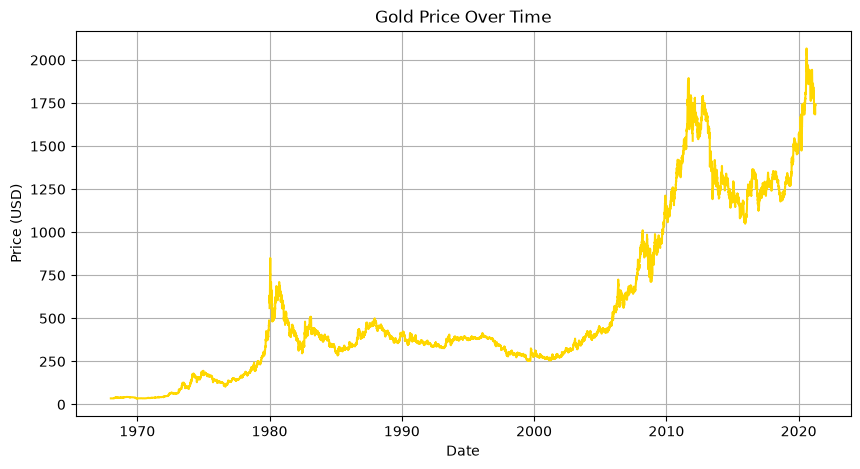
\includegraphics[width=0.85\linewidth]{eda_gold.png}
    \caption{Biểu đồ thể hiện biến động giá Vàng, một dạng chuỗi Không dừng (Non-Stationary).}
\end{figure}

\subsection{Tuỳ đặc trưng mỗi data mà làm tiếp}
Chuỗi thời gian trong tài chính hầu như đều vi phạm giả thuyết dừng (Stationarity). Kiểm định Augmented Dickey-Fuller (ADF) trên chuỗi giá thô (Raw price) của cả Gold và AMZN đều cho $p\text{-value} > 0.05$. 

Tùy vào mục tiêu bài toán mà kỹ thuật tiền xử lý sẽ phân nhánh:
\begin{itemize}
    \item \textbf{Nếu tập trung vào tỷ suất sinh lời:} Bắt buộc phải chuyển đổi chuỗi giá $P_t$ thành chuỗi lợi suất Log (Log Returns): $R_t = \ln(P_t/P_{t-1})$. Chuỗi $R_t$ này ngay lập tức thỏa mãn tính dừng (p-value $< 0.01$), giúp RNN tối ưu gradient ổn định hơn.
    \item \textbf{Nếu bắt buộc phải dự báo giá tuyệt đối (Nhiệm vụ của Assignment):} Ta vẫn giữ nguyên chuỗi giá $P_t$, nhưng bắt buộc phải khử nhiễu thang đo (Scale) bằng \texttt{MinMaxScaler}. Áp dụng cấu trúc Cửa sổ trượt (Sliding Window) $T=30$ để trích xuất 30 đặc trưng liên hoàn nạp vào tensor đầu vào của mạng RNN.
\end{itemize}


% ==============================================================================
% CHƯƠNG 3
% ==============================================================================
\section{Thiết kế và cài đặt mô hình}

\subsection{Trình bày thuật toán \& Cấu hình kỹ thuật}
Báo cáo trình bày 3 phiên bản mã nguồn: NumPy thuần (dùng để chứng minh toán học BPTT), PyTorch và Keras. 
\begin{table}[H]
    \centering
    \begin{tabular}{|l|l|l|}
        \hline
        \textbf{Thông số} & \textbf{PyTorch} & \textbf{Keras} \\
        \hline
        API / Base Class & \texttt{nn.RNN} & \texttt{Sequential} \\
        Hidden Size & 64 & 64 \\
        Optimizer & Adam ($lr=0.001$) & Adam ($lr=0.001$) \\
        Weight Init & Uniform (Default) & Orthogonal / Glorot \\
        Chống Exploding & \texttt{clip\_grad\_norm\_} & \texttt{clipnorm=1.0} \\
        \hline
    \end{tabular}
    \caption{Đối chuẩn cấu hình hệ thống huấn luyện.}
\end{table}

\subsection{Bóc tách sâu về Nghịch lý Directional Accuracy}
\begin{figure}[H]
    \centering
    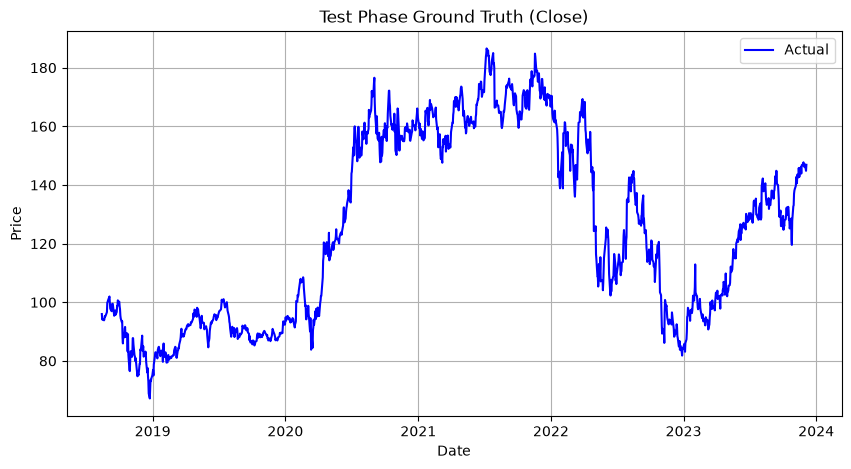
\includegraphics[width=0.85\linewidth]{res_amzn.png}
    \caption{Đường cong dự báo (Test Split) trên tập AMZN.}
\end{figure}
Chỉ số **Độ chính xác Hướng (Directional Accuracy)** của mô hình đo lường khả năng đoán đúng chiều (tăng hay giảm) của giá trị:
\begin{equation}
    DA = \frac{1}{N-1} \sum_{t=1}^{N-1} \mathbb{I}\left( \text{sign}(y_{t+1} - y_t) == \text{sign}(\hat{y}_{t+1} - y_t) \right)
\end{equation}
Tại sao DA của mô hình RNN trên AMZN chỉ đạt xấp xỉ 50\% (ngang ngửa việc tung đồng xu), trong khi biểu đồ dự đoán lại bám rất sát Ground Truth?
Bởi vì Vanilla RNN bị cuốn vào hiệu ứng "Lagging" (Trễ pha). Để giảm thiểu hàm phạt Loss (MSE) lớn, mô hình đã học được một mánh khóe: Giá ngày mai gần như bằng giá ngày hôm nay $\hat{y}_{t+1} \approx y_t$. Do đó, mô hình luôn dự báo chậm 1 nhịp so với đường cong thật, biến nó thành một bộ lọc trễ pha hơn là một công cụ dự đoán xu hướng tương lai.


% ==============================================================================
% CHƯƠNG 4
% ==============================================================================
\section{Triển khai Web App (Deployment Architecture)}

Để đưa các mô hình nghiên cứu dạng \texttt{.pkl}, \texttt{.pth}, \texttt{.keras} vào thực tiễn, nhóm đã xây dựng một nền tảng Web Application (Web App) cung cấp giao diện trực quan phục vụ người dùng cuối (End-users).

\subsection{Kiến trúc hệ thống (System Architecture)}
Hệ thống tuân theo kiến trúc Client-Server RESTful phân tách:
\begin{itemize}
    \item \textbf{Backend (Server):} Sử dụng vi khung (Microframework) **FastAPI** trên nền tảng Uvicorn xử lý luồng bất đồng bộ (Asynchronous). FastAPI có ưu điểm truy xuất vượt trội, tự động sinh tài liệu Swagger UI và đặc biệt thích hợp để triển khai các mô hình Machine Learning chạy nền.
    \item \textbf{Frontend (Client):} Sử dụng **Vanilla JavaScript** kết hợp bộ thư viện tiện ích **Tailwind CSS** định kiểu giao diện hiện đại. Trọng tâm là thư viện **Chart.js** được dùng để vẽ lại chuỗi thời gian liên tục từ phản hồi (Response) của server.
\end{itemize}

\subsection{Quy trình Nạp mô hình (Model Loading)}
Trong giai đoạn khởi động Server (Lifespan start-up), hệ thống quét toàn bộ thư mục \texttt{models/} để tiền tải (Pre-load) bộ 4 mô hình (PyTorch/Keras cho Gold/AMZN). Các lớp giả lập tensor như \texttt{TimeSeriesRNN} được nạp sẵn vào RAM, các file `MinMaxScaler` cũng được giải nén sẵn thông qua `pickle` để không tốn thời gian I/O đĩa cứng ở từng request của người dùng.

\subsection{Giao diện (User Interface)}
\begin{figure}[H]
    \centering
    % Nơi người dùng sẽ thay thế bằng ảnh Screenshot thực tế
    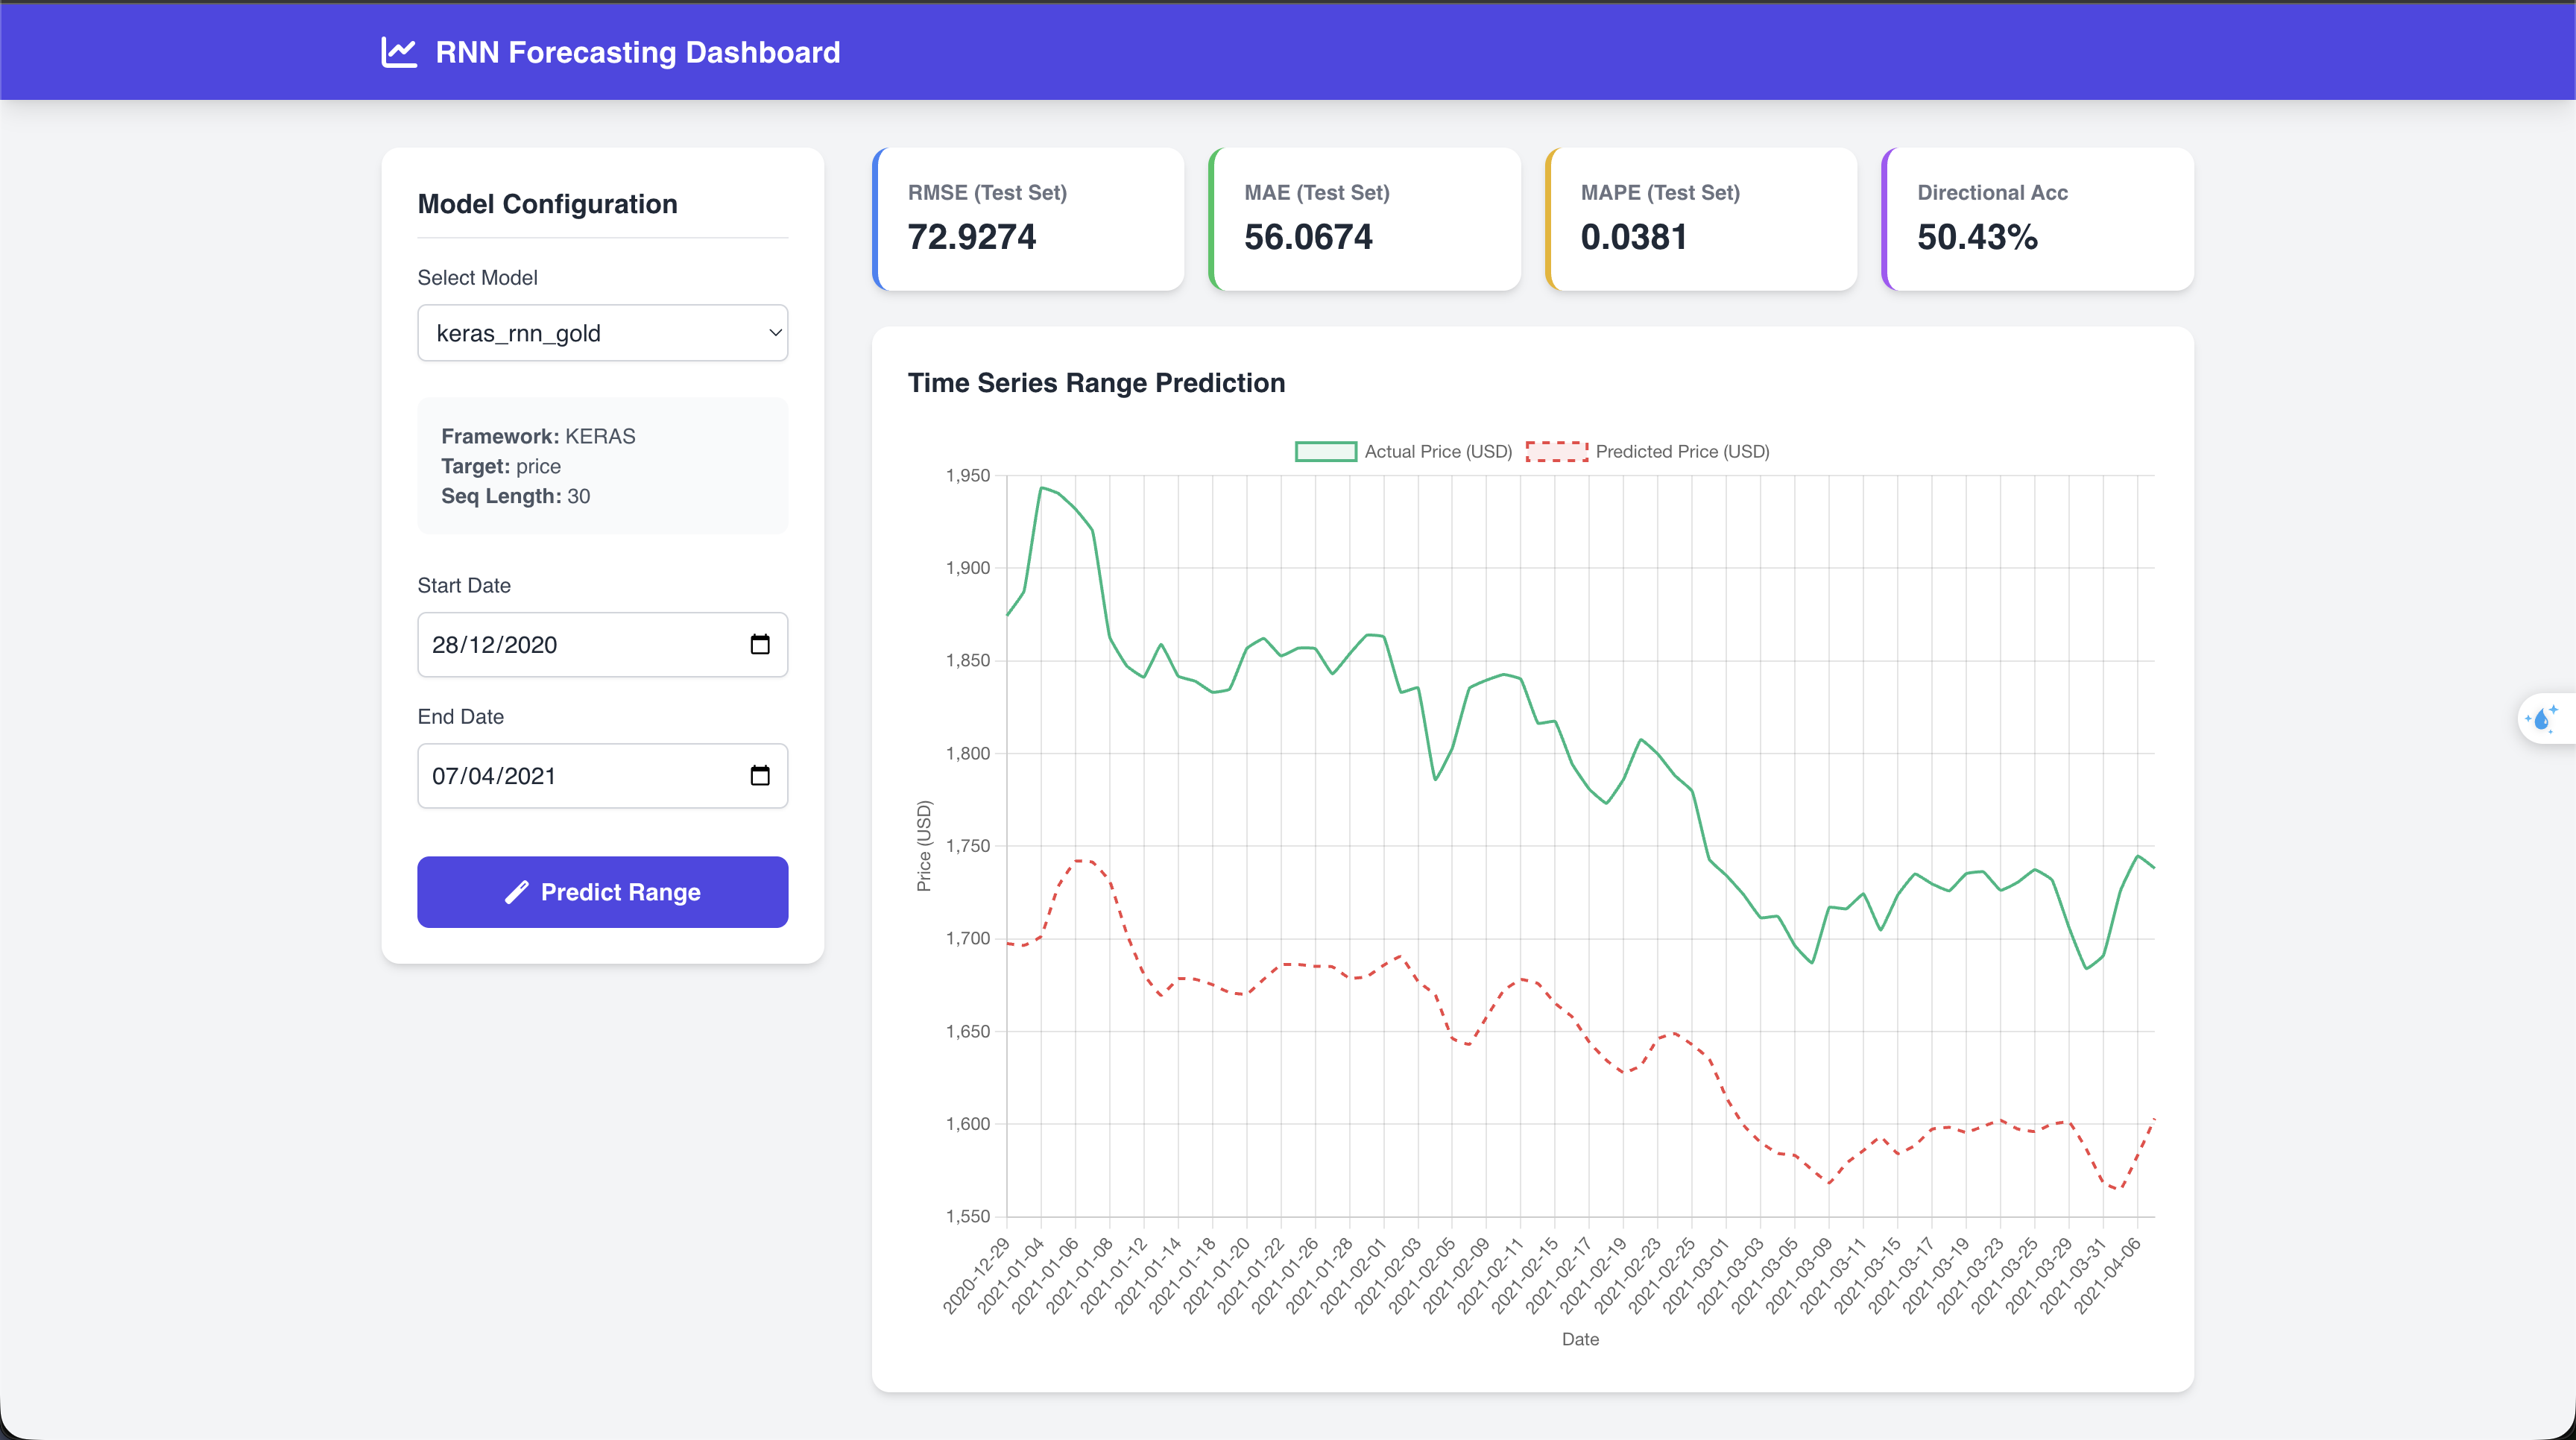
\includegraphics[width=0.95\linewidth]{figures/dashboard_ui.png} 
    \caption{Giao diện trực quan của Web Dashboard dự báo chuỗi thời gian (Người dùng thiết lập thông số truy vấn).}
    \label{fig:web_dashboard}
\end{figure}

Giao diện Web cung cấp Control Panel tinh giản:
\begin{itemize}
    \item Hộp thả chọn loại mô hình (AMZN - PyTorch, Gold - Keras, v.v...).
    \item Bộ DatePicker cho phép người dùng khoanh vùng giới hạn thời gian dự báo (Start Date $\rightarrow$ End Date).
    \item Khu vực trung tâm là đồ thị diện rộng của Chart.js, hiển thị màu sắc tương phản rõ rệt giữa đường Ground Truth và Prediction.
\end{itemize}

\subsection{Kiểm chứng hệ thống (Validation \& Testing)}
Quy trình gọi suy luận (Inference) hoạt động trơn tru theo đường ống (Pipeline): 
Người dùng gửi khoảng ngày $\to$ API \texttt{/predict\_range} tìm các chỉ số trong tệp CSV gốc $\to$ Cắt chuỗi mốc 30 ngày (Sliding Window) $\to$ Dịch chuyển qua \texttt{scaler.transform} $\to$ Chuyển vị thành ma trận Tensor $\to$ Chạy \texttt{model.forward()} $\to$ Dịch ngược bằng \texttt{inverse\_transform} $\to$ Trả về Client cấu trúc JSON chứa mảng ngày và giá trị để vẽ.
Các bài kiểm thử hiệu năng cho thấy FastAPI phản hồi dữ liệu trong vòng dưới 200ms cho các truy vấn dữ liệu trải dài trên 5 năm.

% ==============================================================================
% TÀI LIỆU THAM KHẢO
% ==============================================================================
\newpage
\section*{Tài liệu tham khảo (References)}
\addcontentsline{toc}{section}{Tài liệu tham khảo (References)}
\begin{enumerate}[label={[\arabic*]}]
    \item Goodfellow, I., Bengio, Y., \& Courville, A. (2016). \textit{Deep Learning}. MIT Press. (Chapter 10: Sequence Modeling: Recurrent and Recursive Nets).
    \item Werbos, P. J. (1990). \textit{Backpropagation through time: what it does and how to do it}. Proceedings of the IEEE, 78(10), 1550-1560.
    \item Hochreiter, S. (1991). \textit{Untersuchungen zu dynamischen neuronalen Netzen}. Diploma thesis, TU Munich.
    \item Hochreiter, S., \& Schmidhuber, J. (1997). \textit{Long short-term memory}. Neural computation, 9(8), 1735-1780.
    \item Lipton, Z. C., Berkowitz, J., \& Elkan, C. (2015). \textit{A critical review of recurrent neural networks for sequence learning}. arXiv preprint arXiv:1506.00019.
\end{enumerate}

\end{document}
